\documentclass[11pt,UTF8]{ctexart}
\title{大小大流体在库埃特与泊肃叶流下的数值模拟情况}
\author{马坤}
\date{2020.1.7}
\usepackage{amsmath}
\usepackage{graphicx}
\usepackage{caption}
\usepackage{subcaption}
\usepackage[left=1in, right=1in, top=1in, bottom=1in]{geometry}
\begin{document}
    \maketitle
    \par{大小大流体指的是管道中第一层为粘性较大的流体,第二层为粘性较小的流体,
    第三层为粘性较大的流体。假设我们模拟的区域高度为$H=1$(同样假设模拟区域长度
    $L=1$),那么有刻画流体
    区域的示性函数$\phi$:}
    $$
    \phi=
    \begin{cases}
        0.5[-\tanh{\frac{y-1/3}{W}}+1],\text{$y\leq H/2$}\\
        0.5[\tanh{\frac{y-2/3}{W}}+1],\text{$y>H/2$}
    \end{cases}
    $$
    \par{$\phi$理应($W$较小)粘性较大流体里面
    ($y < H/3$ 或者 $y > 2H/3$)为1,理应($W$较小)在粘性较小流体里面$(H/3 < r < 2H/3)$为0。}
    \par{模拟中我们假设粘性比$\frac{\eta_s}{\eta_l}=rate$,其中$\eta_s$为较大的粘性,无维
    度化后的粘性系数$\eta$有如下表达式:
    $$\eta = 1+rate*\phi-\phi.\eqno(2)$$
    上述两个表达式上面两个表达式中的$W,rate$都是待定的参数,接下来会通过实验
    选取较好的值。实验中假设的流体的密度均为$\rho=1$,所以有$\eta=\nu$。}
    \section{库埃特流}
    \par{在这一节中我们将考察库埃特流,即上面板具有速度,假设为$u_{up}=0.1$,下
    面板速度为$u_{bottom}=0$。流体流动的过程中我们不考虑外力。第一小节是改变$W$,
    第二小节为改变$rate$。}
    \subsection{改变$W$}
    \par{如果只考虑单一流体,那么流体的流速应该为线性增长的,但是本文考虑的为大小
    大流体模型,所以流速图会有所差异。此小节的实验,选用的$rate=50$,对照黄老
    师论文,我们选取了$Re=500$。}
    \begin{figure}[h]
        \centerline{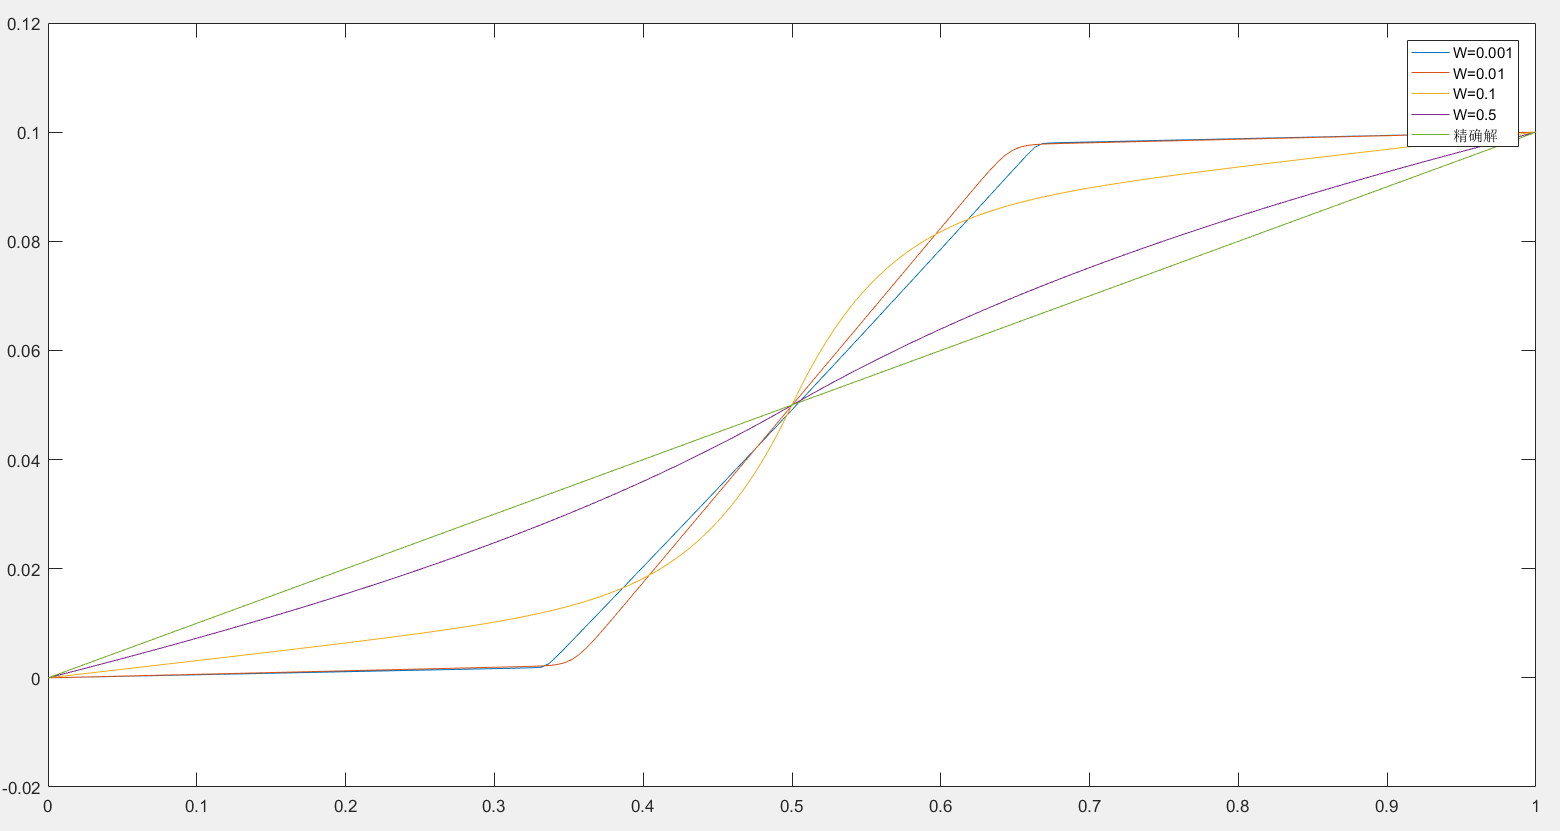
\includegraphics[width=0.8\textwidth]{cutte_W.png}}
        \caption{库埃特流随着$W$变化的图像}
    \end{figure}
    \par{观察图片可见,当$W$较大时流速趋于一条直线,尤其是$W=0.5$。这是因为当
    $W$过大时,示性函数$\phi$已经不能较好的反应流体的性质了,这导致了流体粘性比
    小于希望的值;而当$W$较小时示性函数$\phi$较好的反应了流体的性质。观察$W=0.001$
    图像,靠近下面板的大粘性流体速度几乎为0,而靠近上面板的流速为近似为0.1,
    可以理解为粘性大的流体和面板粘在一起。}
    \subsection{改变$rate$}
    \par{此小节我们选取的$W=0.01$,然后考察流体稳定后的流速与$rate$之间的关系。
    此时,虽然改变了$rate$的值,按照黄老师的对应关系,$Re$也应该改变,但是这里
    仍然固定$Re=500$.可以看见当流体粘性比越小时,流速越趋于一条直线,这和我们的
    理解是相同的。当$rate=1$时,无维度$\eta$就是一个常数,与位置无关,此时画
    出来图片理应为一条直线,与库埃特流精确解一致。但是由于解收敛太慢了,达到此
    过程之前就最大时间停机了。}
    \begin{figure}[h]
        \centerline{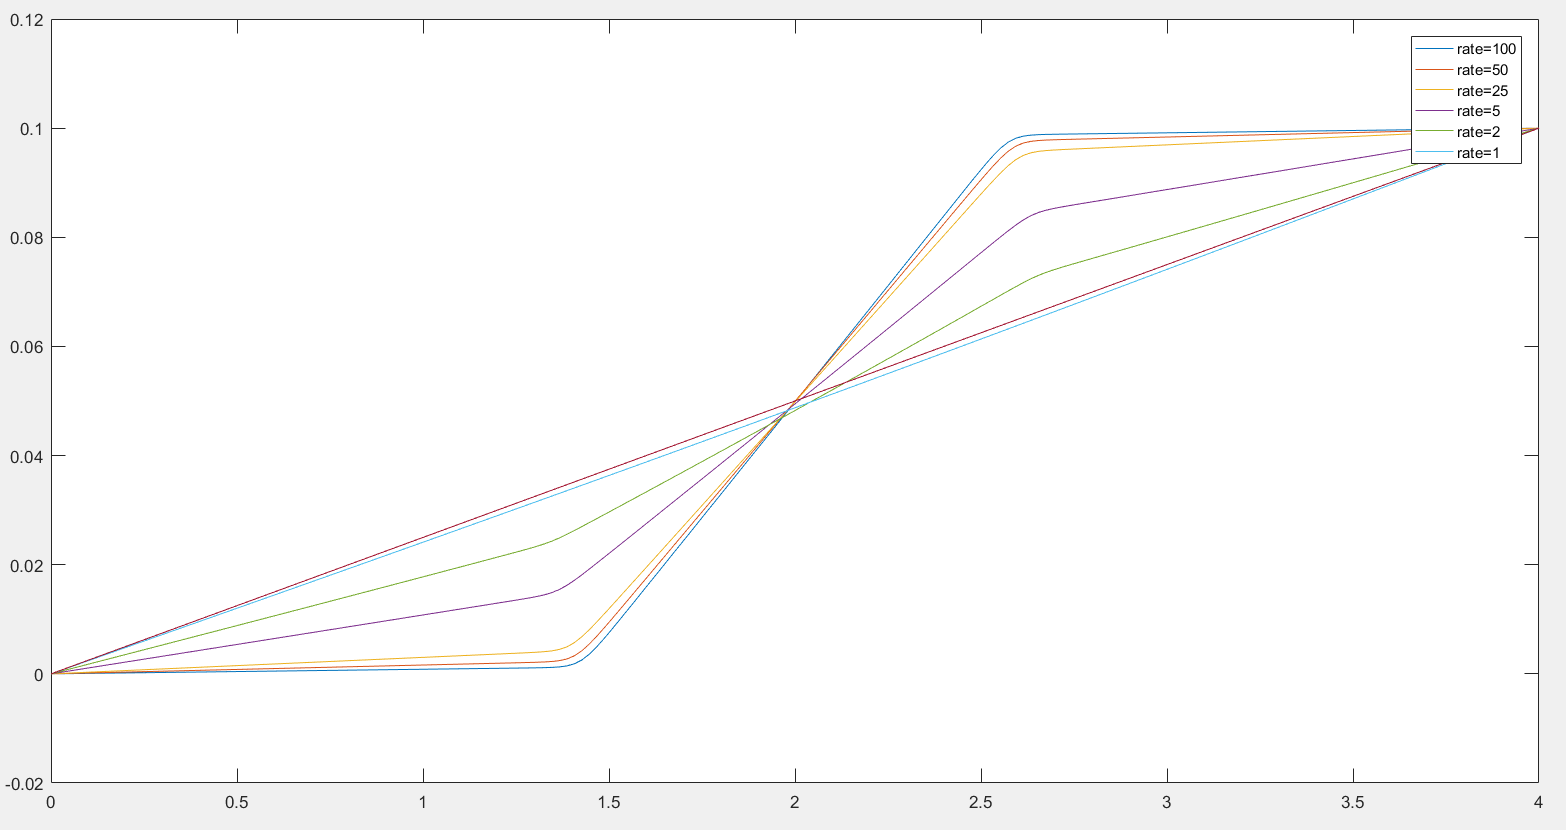
\includegraphics[width=0.8\textwidth]{cutte_rate.png}}
        \caption{库埃特流随着$rate$变化的图像}
    \end{figure}
    \section{泊肃叶流}
    \par{在这一节中我们将考察泊肃叶流,即上下面板没有速度,$u_{up}=u_{bottom}=0$。
    流体流动的过程中我们考虑外力,其中我们外力的选取为$F=\frac{8\rho u_{peak} \eta_s}{H^2}$,其中$u_{peak}=0.1$。如果是单一成分流体,
    并且流体的粘性为$\eta_s$,那么流速应该是一个抛物线,并且峰值为0.1。同样的,
    第一小节是改变$W$,第二小节为改变$rate$。}
    \subsection{改变$W$}
    \par{同库埃特流一样,当$W$较大时流速趋于一条抛物线,尤其是$W=0.5$,但是峰值
    不是0.1。这是因为当$W$过大时,示性函数$\phi$已经不能较好的反应流体的性质了,
    这导致了流体粘性比小于希望的值,图像进而类似抛物线,而峰值不为0.1的原因为我们
    外力相对于粘性小的流体来说太大了;而当$W$较小时示性函数$\phi$较好的反应了流体
    的性质。随着$W$的减小,大粘性流体的速度趋于精确解,但小粘性的流体的流速却不停
    的增大,也许会稳定下来。}
    \begin{figure}[h]
        \centerline{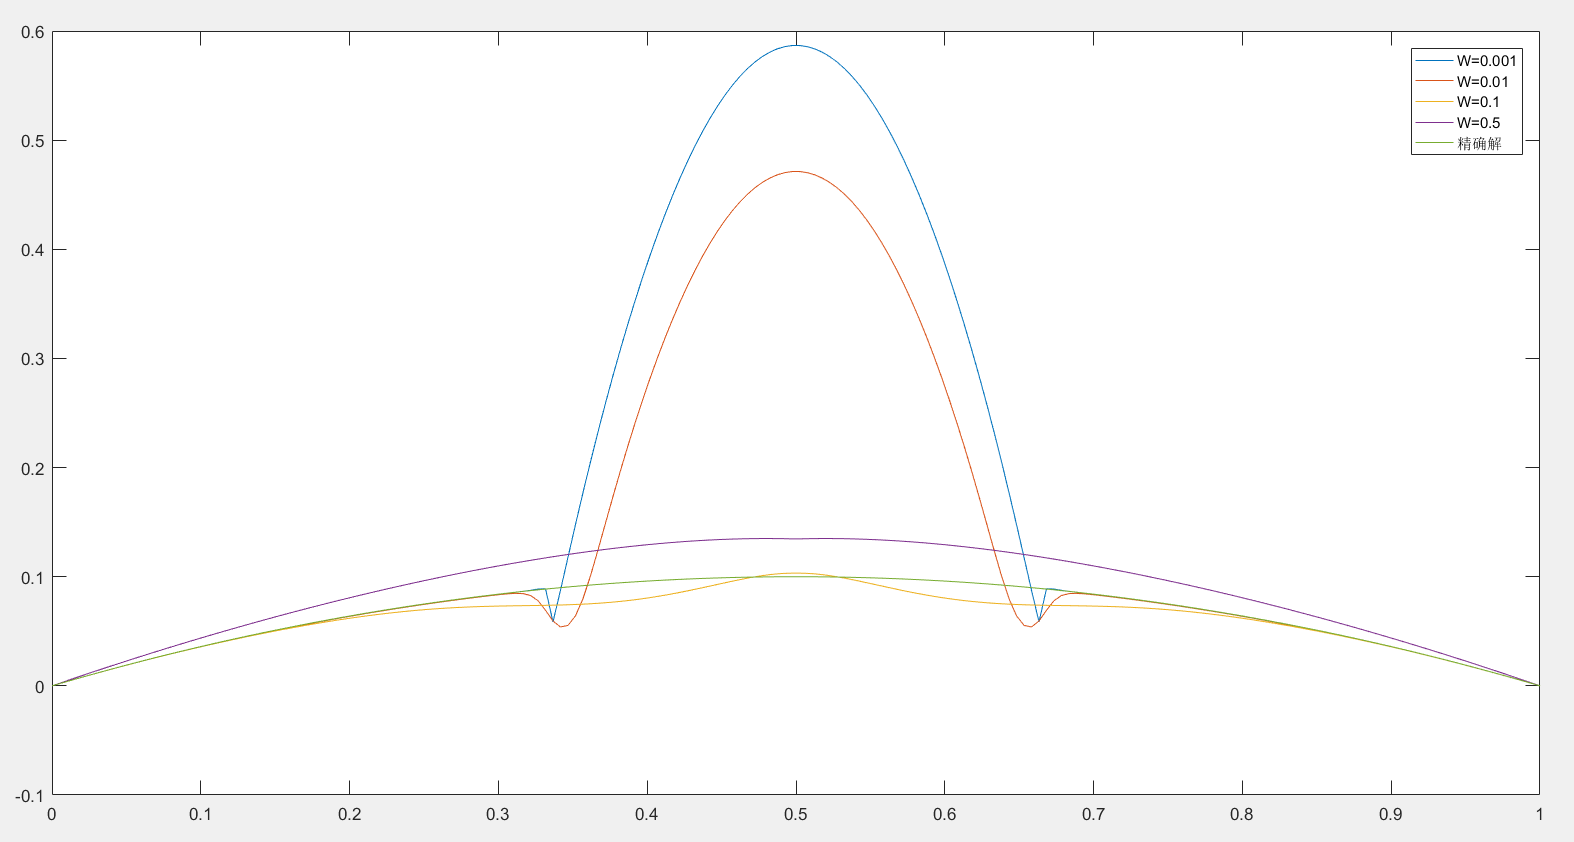
\includegraphics[width=0.8\textwidth]{Poiseuille_W.png}}
        \caption{泊肃叶流随着$W$变化的图像}
    \end{figure}
    \subsection{改变$rate$}
    \par{此图的参数选取与库埃特流的第二小节一样,$Re=500,W=0.1$,不过我们这里改变
    了$rate$,所以进而力也会改变。这个图像就不那么好理解了,尤其是$rate=100$时,
    流体流速很反常。但还是当我们取$W=0.01$时,情况有所变化。}
    \begin{figure}[h]
        \centerline{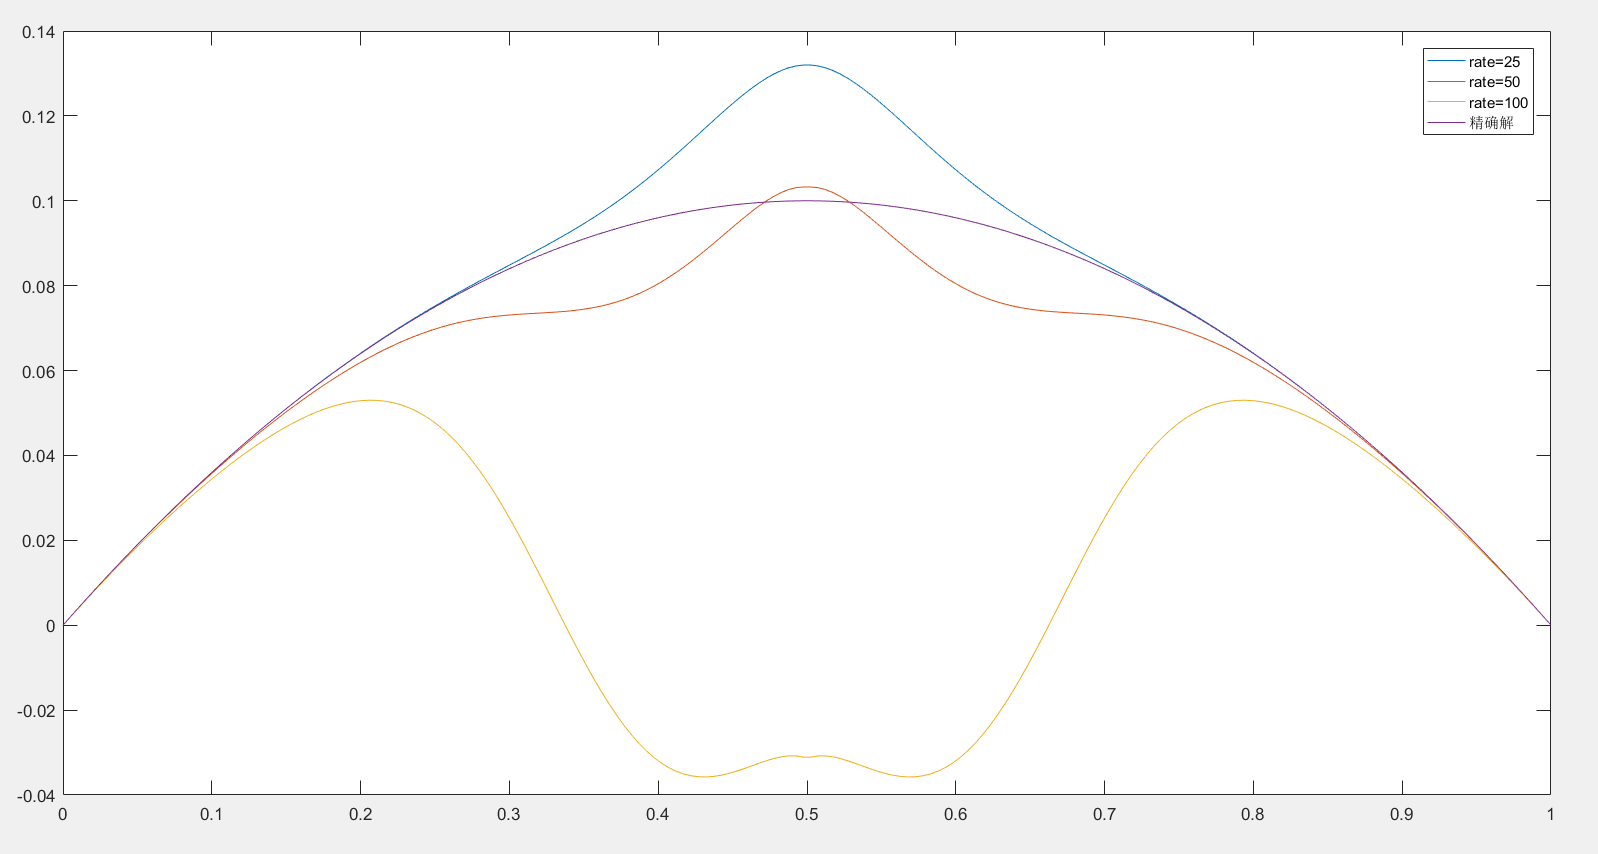
\includegraphics[width=0.8\textwidth]{Poiseuille_rate_W_0_1.png}}
        \caption{泊肃叶流随着$rate$变化的图像($W=0.1$)}
    \end{figure}
    \begin{figure}[h]
        \centerline{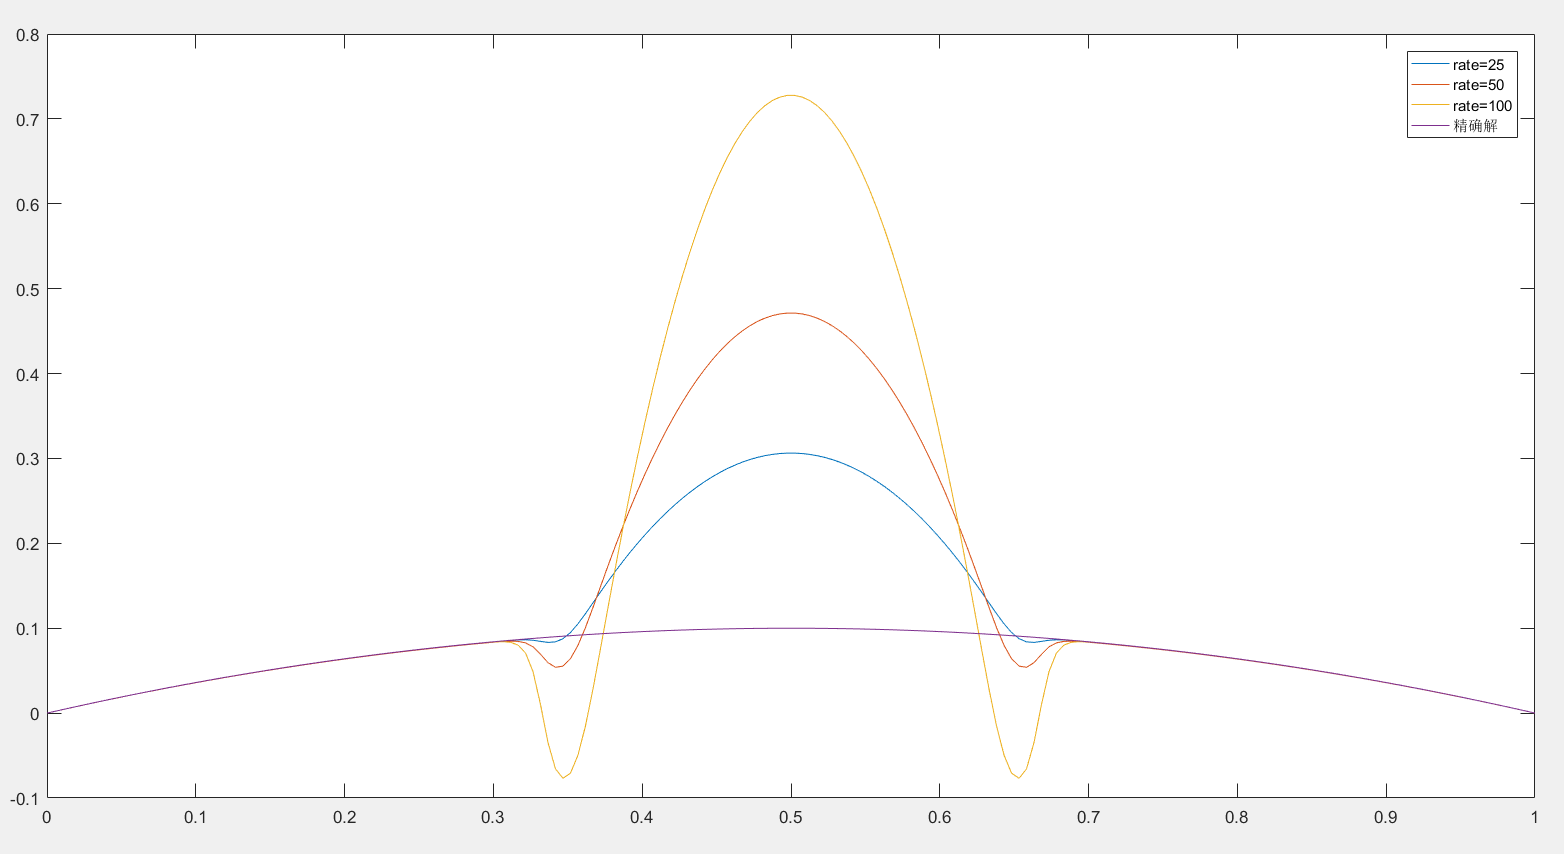
\includegraphics[width=0.8\textwidth]{Poiseuille_rate_W_0_01.png}}
        \caption{泊肃叶流随着$rate$变化的图像($W=0.01$)}
    \end{figure}
\end{document}